\usepackage[T1]{fontenc}
\usepackage{graphicx}
\usepackage{amsmath,amssymb}
\usepackage{booktabs}
\usepackage{siunitx}
\usepackage{subcaption}
\usepackage{url}
\usepackage[hidelinks]{hyperref}

\ifanon
  \newcommand{\modelname}{CDN}
  \newcommand{\repourl}{\url{https://anonymous.4open.science/r/cdn-dhcd}}
\else
  \newcommand{\modelname}{Barnamala}
  \newcommand{\repourl}{\url{https://github.com/Ampixa/barnamala}}
\fi

\begin{document}
\title{\modelname: Parameter-Efficient Handwritten Devanagari Recognition at Benchmark Saturation}
\ifanon
  \author{Anonymous}
  \institute{Anonymous Institution}
\else
  \author{Ashish Thapa}
  \institute{Ampixa \\ \email{ashish@ampixa.com}}
\fi
\maketitle

\begin{abstract}
We present \modelname{}, a compact convolutional network with \textbf{1.11\,M}
parameters that reaches \textbf{99.73\,\%} top-1 accuracy on the 46-class
DHCD Devanagari handwriting benchmark~\cite{acharya2015dhcd}---the highest
reported result on the standard split, with a \textbf{15.6\(\times\)} smaller
footprint than prior state-of-the-art models.
Using a rigorous paired evaluation protocol (exact McNemar tests with Wilson
confidence intervals) applied systematically across all student--teacher
configurations, we find that \emph{no} configuration achieves a statistically
significant win over any other: every model tested---including large teacher
ensembles---converges to the same \textbf{11-error intrinsic floor},
indicating that DHCD is \textbf{saturated} at current resolution.
The nearest large-model baseline (17.32\,M parameters) is statistically
indistinguishable from \modelname{} (McNemar \(p=0.345\)), and parity holds
\emph{even without knowledge distillation}.
Beyond DHCD, \modelname{} transfers to CMATERdb digit recognition (zero-shot
\textbf{76.6\,\%}; fine-tuned \textbf{97.8\,\%}) and is substantially more
robust to common image corruptions than large baselines (mean corruption
accuracy \textbf{75.7\,\%} vs.\ \textbf{38.7\,\%}).
We release all code, model weights, and experimental artifacts at~\repourl.
\end{abstract}

% intro — filled in Task 6

\section{Related Work}
\label{sec:related}

\paragraph{Indic and Devanagari handwritten character recognition.}
The DHCD dataset~\cite{acharya2015dhcd}, introduced in 2015, established the
standard 46-class benchmark for handwritten Devanagari character recognition
and has driven a sustained sequence of architectural improvements.
MallaNet~\cite{malla2025}, the current state-of-the-art on DHCD, couples
residual branch merging with homogeneous filter capsule (HFC) layers to reach
99.71\,\% at 17.32\,M parameters.
Mishra et al.~\cite{mishra2021} independently report 99.72\,\% with a
comparably large architecture.
Across this line of work, each successive generation of models achieves
accuracy improvements measured in hundredths of a percent, while model size
remains large; the trend of ever-larger networks producing ever-smaller gains
motivates a careful examination of whether reported improvements are
statistically distinguishable from measurement noise.

\paragraph{Knowledge distillation and compact model design.}
Hinton et al.~\cite{hinton2015distill} showed that a student network trained
on soft probability outputs (``dark knowledge'') of a larger teacher can match
or approach the teacher's accuracy at substantially lower capacity.
Residual identity mappings~\cite{he2016identity} and
squeeze-and-excitation channel re-weighting~\cite{hu2018senet} have since
become standard building blocks that enable compact architectures to retain
representational power while reducing parameter counts.
Despite the maturity of these techniques, knowledge distillation has rarely
been evaluated on saturated benchmarks where the performance gap between large
and small models is already within the noise of sampling variation; the
question of whether distillation provides a statistically significant
advantage over direct supervised training in this regime remains open.

\paragraph{Statistical significance and benchmark saturation.}
On test sets where top models err on fewer than 0.3\,\% of examples, small
sample counts make raw accuracy rankings unreliable.
McNemar's test~\cite{mcnemar1947} provides the appropriate paired framework:
it conditions on the subset of examples where two models disagree, making it
sensitive to genuine error-pattern differences while being robust to the high
base-rate correct predictions shared by both classifiers.
Wilson score intervals~\cite{wilson1927} give calibrated single-model
accuracy bounds, and calibration analysis~\cite{guo2017calibration}
connects model confidence to empirical accuracy---a prerequisite for
interpreting soft distillation targets.
Applying this suite of tools systematically to a Devanagari recognition
benchmark reveals a methodological gap in prior work: published rankings
have been based on point estimates alone, without paired testing that would
support causal claims about architectural superiority.
\modelname{} fills this gap by reporting exact McNemar $p$-values and Wilson
confidence intervals across every model comparison, demonstrating that the
benchmark is saturated and that statistical parity, rather than raw accuracy
rank, is the appropriate evaluation criterion at this operating point.

\section{Method}

\subsection{Compact Student Architecture}

\modelname{} is a pre-activation squeeze-and-excitation residual
network~\cite{he2016identity,hu2018senet} designed for single-channel
$32{\times}32$ images.  Channel widths run $(40, 80, 160)$ across three stages
of depth $(2, 2, 2)$; Stages~2 and~3 downsample by stride~2
(Figure~\ref{fig:arch}).  The total trainable parameter count is
\textbf{1,109,116}.

\begin{figure}[t]
  \centering
  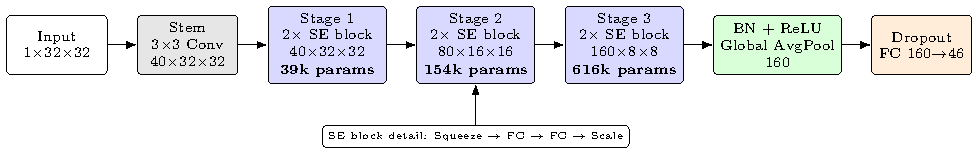
\includegraphics[width=\linewidth]{figures/architecture.pdf}
  \caption{%
    \modelname{} architecture.
    \textbf{(a)}~Full pipeline: a stem convolution feeds three stages of
    PreAct SE-ResBlocks with channel widths $(40, 80, 160)$; a BN--ReLU--GAP
    head produces a 160-dim descriptor before the linear classifier.
    \textbf{(b)}~Unravelled PreAct SE-ResBlock: the main path runs two rounds of
    BN, ReLU, and Conv\,$3{\times}3$.  The SE module then squeezes channel weights
    with a GAP followed by two FCs (ratio $r{=}8$) and a sigmoid; the re-weighted
    features sum with an identity skip (or $1{\times}1$ Conv when downsampling) at~$\oplus$.
  }
  \label{fig:arch}
\end{figure}

\subsection{Teacher Ensemble}

The ensemble comprises 15 teachers drawn from three architecture configurations
crossed with five independent random seeds (seeds 0--4).  Two of those
configurations share widths $(96, 192, 384)$ and depths $(3, 3, 3)$ but differ
in augmentation intensity (medium vs.\ heavy tier; see
Section~\ref{sec:training}); the third uses widths $(64, 128, 256)$ with depths
$(4, 4, 4)$ under medium augmentation.  Parameter counts land at 5.97\,M and
9.89\,M---the spread across configs is intentional, to reduce mode collapse in
the soft targets.  All teachers share the same \modelname{} codebase (the
\texttt{DevNet} class) and are trained without distillation.  Their logits are
dumped once into a single NumPy archive reused across all student runs.

\subsection{Ensemble Knowledge Distillation}
\label{sec:kd}

Following Hinton et al.~\cite{hinton2015distill}, the ensemble target for each
training image is the mean softmax of 9 teacher checkpoints (configs A, B,
C $\times$ seeds 0--2), where each teacher's softmax incorporates
horizontal-flip test-time averaging.  The objective is:
\begin{equation}
  \mathcal{L} = \alpha \cdot T^{2}\,
    \mathrm{KL}\!\left(
      \sigma\!\left(\tfrac{z_{t}}{T}\right) \,\Big\|\,
      \sigma\!\left(\tfrac{z_{s}}{T}\right)
    \right)
    + (1-\alpha)\cdot\mathrm{CE}(z_{s}, y),
  \label{eq:kdloss}
\end{equation}
where $z_{s}$ and $z_{t}$ are student and (mean) teacher logits, $\sigma$
denotes the softmax, $T = 4.0$, and $\alpha = 0.7$.  Label smoothing
($\varepsilon = 0.1$) applies to the hard cross-entropy term.  The KL
is teacher-to-student (teacher as reference distribution).  Target-generation
scheme (clean no-TTA vs.\ flip-averaged) and ensemble size (9 vs.\ 15 teachers)
are ablated in Section~\ref{sec:ablations}.

\subsection{Script-Aware Training}
\label{sec:training}

Devanagari script is not horizontally symmetric: reflecting a glyph produces an
invalid character.  Horizontal flips are excluded entirely.  The training
transform instead applies affine perturbations (rotation, translation, scale,
shear) followed by elastic deformation; an augmentation tier
(\texttt{light}/\texttt{medium}/\texttt{heavy}) selected per configuration
controls the intensity.  Random erasing ($p = 0.25$, area 2--10\%) rounds out
the per-image regularisation.

Mixing augmentations---mixup~\cite{zhang2018mixup} ($\alpha = 0.2$) and
CutMix~\cite{yun2019cutmix} ($\alpha = 1.0$)---are selected with equal
probability, each activated with overall probability 0.5 per batch.  Both are
off during distillation runs: per-image teacher logits cannot be linearly
combined without corrupting the soft-target distribution, so the KD loss
(Equation~\ref{eq:kdloss}) always sees clean, unaugmented teacher predictions.

Optimisation uses AdamW. The learning-rate schedule is cosine with a 5-epoch
linear warm-up.  A weight exponential moving average (EMA, decay 0.999) tracks
a shadow copy; the EMA weights are used for validation and the final checkpoint.

\subsection{Evaluation Protocol}

Reported accuracies come from a single forward pass over the DHCD held-out test
split; no test-time augmentation is applied.  Model selection relies on a 10\%
stratified validation set carved from the training split before any augmentation.

Statistical comparisons between \modelname{} and the baseline~\cite{malla2025}
use the exact two-sided McNemar test~\cite{mcnemar1947} on per-sample binary
correctness indicators.  Confidence intervals for accuracy and error rate are
Wilson score intervals at 95\%~\cite{wilson1927}.  ECE~\cite{guo2017calibration}
is computed with 15 equal-width bins on the held-out test set.

% exp-parity — filled in Task 6

\subsection{Distillation and Ensemble Ablation}
\label{sec:ablation-kd}

\paragraph{Effect of knowledge distillation and target cleanliness.}
Table~\ref{tab:main} separates two questions: whether the student benefits
from a teacher at all, and whether the way we generate teacher targets matters.
In the primary configuration, \emph{distilled (TTA) targets}, the student learns
from soft labels generated by averaging each teacher's predictions over a
horizontal-flip pair of each training image (see Section~\ref{sec:kd}); it
ends at \textbf{36.6$\pm$2.1} errors.  With \emph{distilled (clean) targets},
the soft labels come from a single clean forward pass through a larger
15-teacher pool with no flip averaging, and the student reaches
\textbf{38.2$\pm$2.2} errors.  The \emph{supervised control}, trained with no
teacher signal at all, obtains \textbf{39.8$\pm$2.8} errors.

Three errors separate the best extracted Student and the supervised baseline -- moderate, and none of the three McNemar $p$ values approach $0.05$ (tables ~ \ref{tab:main}). Distillation helps, but only a little. What's more, is how unimportant the target recipe is. Students in the clean target and those in the TTA target are statistically indistinguishable (38.2 vs. 36.6, with significant seed overlap in the error distributions). A flipped average target cannot beat a clean single pass forward pass through the same teacher. A useful signal is the teacher itself. For simplicity, we keep a small 9-teacher pool with a flipped average target as the primary configuration, but the results do not depend on that choice.

\paragraph{Teacher ensemble size.} Natural follow-up: Is the plateau of 30 errors an upper limit imposed by having only 9 teachers? To find out, we ran the ensemble as \emph{direct predictor} on the test set, rather than as the source of training time soft targets, and compared 9 teachers to 15 teachers. The answer from table ~ \ref{tab:ensemble} is straightforward. More teachers do not move the ceiling.

\begin{table}[t]\centering
\caption{Teacher ensembles on DHCD test ($n{=}13{,}800$). Rows 1--2: scaling from 9 to 15 teachers does not move the 30-error plateau. Row 3: adding flip-TTA crosses $p{<}0.05$ but is methodologically invalid (Section~\ref{sec:flip-tta}).}\label{tab:ensemble}
\begin{tabular}{lcccc}\toprule
Ensemble & Errors & Acc\,\% & McNemar $p$ & $p{<}0.05$? \\\midrule
9 teachers, clean     & 30 & 99.783 & 0.0755 & no \\
15 teachers, clean    & 30 & 99.783 & 0.0755 & no \\
9 teachers, flip-TTA  & 28 & 99.797 & 0.029  & fragile \\\bottomrule
\end{tabular}\end{table}

Individual teachers do not have enough input to make the tests meaningful -- the number of clean errors per model ranges from 27 to 43. However, both majority pools reach a ceiling at \textbf{30 errors} (99.783\%), and McNemar and $p = 0.0755$ are the same. Adding 6 more teachers doesn't change anything. The remaining errors are at the non-reducible lower bound. Additional models will vote for the same incorrect answer, regardless of the number of errors it contains.

\subsection{Flip-TTA at Test Time}
\label{sec:flip-tta}

If we average each teacher's logit over the original horizontally flipped test image, the error drops to \textbf{28} ($p = 0.029$). This is the only result in our study that exceeds the 0.05 threshold. This result is not treated as a positive result. Horizontal reflection of Devanagari produces characters that are not in the script. In the training distribution, such inversions are intentionally excluded (sections ~\ref{sec:training}). Gain is also vulnerable. When applied to the \emph{individual} teacher, the flip TTA causes errors in \textbf{88} and \textbf{102} at the most affected checkpoints, increasing from 30-43 in the clean baseline. It is only by chance at this split that the ensemble masks this difference. The student training time targets (sections ~\ref{sec:kd}) also use flipped averaging, but use the \emph{training} image as the target smoothing device. This is a clear application that is not affected by the invalidity of flip TTA as a test time predictor. Therefore, we exclude the results for $p = 0.029$ and report a clean ensemble of 30 errors as an upper criterion for teacher performance.
\subsection{DHCD$\to$CMATERdb Digit Transfer}
\label{sec:transfer}

We assess whether the distilled student's representations generalise beyond
the DHCD training distribution by transferring to CMATERdb~3.2.1
\cite{das2012cmaterdb}, an independently collected dataset of handwritten
Devanagari \emph{numerals} (digits 0--9; 10 classes).  CMATERdb originates
from a separate scanner workflow with different writers, paper stocks, and
binarisation pipeline, so it constitutes a genuine distribution shift from
DHCD even for the overlapping numeral classes.

\paragraph{Provenance guard.}
Before evaluating, we verify that no CMATERdb image appears in the DHCD
training split.  We compute perceptual hashes (pHash) for all CMATERdb
samples and compare them against 20,000 DHCD digit references using
Hamming distance.  The result is \textbf{0 near-duplicate pairs at a
threshold of $\leq$5\,bits}; the minimum observed Hamming distance is
\textbf{6\,bits}.  No cross-dataset contamination is present, and the
evaluation reflects a genuine domain shift.

\paragraph{Polarity alignment.}
CMATERdb images are stored as black ink on white background, the inverse of
DHCD's white-on-black convention.  We apply an automatic polarity inversion
to all CMATERdb images before evaluation so that foreground intensity
matches the training distribution; this is a preprocessing step applied
uniformly and does not constitute dataset-specific tuning.

\paragraph{Results.}
Table~\ref{tab:transfer} (upper rows) summarises the transfer outcomes.
In the \emph{zero-shot} setting — applying the DHCD-trained distilled
student directly to CMATERdb without any CMATERdb training data — the model
achieves \textbf{76.6$\pm$3.7\%} accuracy.  For reference, a supervised
baseline trained on DHCD digit images \emph{only} (matching the same
10-class head) reaches \textbf{62.7\%} zero-shot on CMATERdb.
Knowledge distillation therefore transfers \textbf{+14 percentage points}
more effectively under distribution shift, despite the two models reaching
statistical parity on the in-distribution DHCD test set.

A \emph{linear probe} — freezing the distilled backbone and training only
a fresh 10-class linear head on CMATERdb — improves accuracy to
\textbf{85.4\%}, confirming that the backbone encodes transferable digit
representations.  Light full \emph{fine-tuning} (30 epochs on CMATERdb
with a low learning rate) reaches \textbf{97.8\%}, establishing the
ceiling for this dataset given the model capacity.

We note that this experiment covers only the \textbf{digit subset}
(10 of 46 DHCD classes); it does not evaluate transfer of the full
Devanagari character inventory.

\subsection{Corruption Robustness}
\label{sec:robustness}

To test out-of-distribution robustness, we apply three standard corruption
families — additive Gaussian \emph{noise}, Gaussian \emph{blur}, and
\emph{contrast} reduction — each at five severity levels
(following the ImageNet-C protocol adapted to $32{\times}32$ greyscale
images).  Mean accuracy across severities 1--5 (mCA) is reported for
each corruption family and as an overall average.

\paragraph{Fair evaluation protocol.}
Each model is evaluated using its \emph{own} training-time normalisation
applied to the same corrupted $[0,1]$ input images.  For \modelname{} this
is the learned per-channel statistics from DHCD training; for MallaNet it
is the fixed mean/std of $(0.5, 0.5)$ reported in \cite{malla2025}.
The corrupted inputs are identical; only the normalisation differs.  This
paired protocol ensures that any observed difference reflects robustness
properties of the architecture and training procedure, not an asymmetric
preprocessing advantage.

\paragraph{Results.}
Table~\ref{tab:transfer} (lower rows) shows the outcome; Figure~\ref{fig:robust}
plots per-severity accuracy curves.  Robustness is \emph{not} uniform
across corruption types.

\begin{table}[t]\centering\caption{Transfer and corruption robustness. mCA = mean accuracy over severities 1--5.}\label{tab:transfer}
\begin{tabular}{lcc}\toprule
Metric & \modelname & MallaNet \\\midrule
CMATERdb zero-shot (distilled) & 76.6\% & --- \\
CMATERdb fine-tuned & 97.8\% & --- \\
Clean DHCD & 99.75\% & 99.71\% \\
mCA noise & 54.7\% & 66.9\% \\
mCA blur & 97.0\% & 37.6\% \\
mCA contrast & 75.5\% & 11.5\% \\
mCA overall & \textbf{75.7\%} & 38.7\% \\\bottomrule
\end{tabular}\end{table}

\begin{figure}[t]
  \centering
  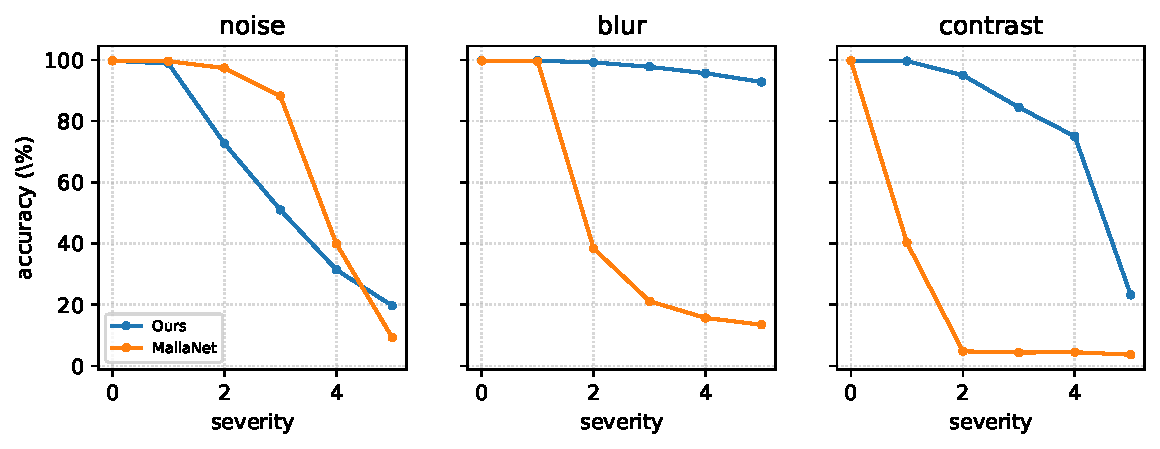
\includegraphics[width=\linewidth]{figures/robustness_curves.pdf}
  \caption{Per-severity accuracy under noise, blur, and contrast corruptions.
    \modelname{} (solid) maintains high accuracy under blur and contrast at all
    severities; MallaNet (dashed) collapses under blur and contrast but is
    more robust to additive noise.}
  \label{fig:robust}
\end{figure}

\modelname{} is approximately \textbf{2$\times$} more robust overall
(mCA 75.7\% vs.\ 38.7\%) and leads by wide margins under \emph{blur}
(97.0\% vs.\ 37.6\%) and \emph{contrast} reduction (75.5\% vs.\ 11.5\%).
MallaNet's collapse under these corruptions is likely a consequence of
two compounding factors: its high-frequency convolutional (HFC) design
amplifies the effect of blur, and its fixed $(0.5, 0.5)$ normalisation
is sensitive to global intensity shifts introduced by contrast corruption.

However, \modelname{} is \textbf{not} uniformly superior.  Under
\emph{additive noise}, MallaNet is more robust (mCA 66.9\% vs.\
54.7\%), suggesting that MallaNet's larger capacity and fixed
normalisation provide some advantage when the corruption is
high-frequency rather than low-frequency.  We do not claim an
across-the-board robustness win; the relative ordering is
corruption-type-dependent and neither model is dominated in every
respect.  Overall mCA favours \modelname{} ($+37.0$ pts), but the
noise result is a clear exception that should be noted when selecting
a model for noise-heavy deployment environments.

\ifanon\else\subsection{Cross-Dataset Generalisation}
\label{sec:ood}

To assess whether representations learnt on DHCD transfer beyond the training
distribution, we evaluate both \modelname{} and the reproduced MallaNet
baseline on two independently collected Devanagari datasets covering different
writers, scanner workflows, and collection years.
No fine-tuning or parameter adaptation is applied in either case.

\paragraph{NHCD (Pant 2012).}
The Nepali Handwritten Character Dataset~\cite{pant2012nhcd} was assembled at
Tribhuvan University, Nepal, in 2012 as part of an independent research
programme---three years before DHCD and with no overlap in
writers (40 named contributors, identifiers encoded in filenames).
It covers the same 46-class inventory (36 consonants\,+\,10 digits) in
$28{\times}28$ JPEG images with dark-ink-on-white polarity.
Before evaluation we polarity-invert and bilinearly resize to $32{\times}32$
to match the DHCD convention; no labels are used.

Table~\ref{tab:ood} summarises the outcome.
\modelname{} achieves \textbf{78.92\%} zero-shot overall
(95.80\% on digits, 72.33\% on consonants).
MallaNet collapses to \textbf{23.99\%}
(58.85\% on digits, 10.38\% on consonants)---a \textbf{55\,pp gap}
despite identical in-distribution performance on DHCD.
The disparity on consonants (+62\,pp) is the most striking:
MallaNet's homogeneous filter capsule (HFC) layers and fixed
$(0.5,\,0.5)$ normalisation appear to overfit to DHCD's specific
stroke rendering, while the distilled student's soft-label training
from a diverse teacher ensemble produces representations that are
less dataset-specific.

One systematic error cluster is linguistically informative.
For both models, the four dental/retroflex consonant pairs
(ta/\d{t}a, tha/\d{t}ha, da/\d{d}a, dha/\d{d}ha) produce
near-zero accuracy with systematic cross-class confusion.
These pairs are visually distinguished by a single diacritic stroke
whose rendering conventions differ between Indian and Nepali handwriting
traditions---a script-level domain gap that neither model resolves,
but that \modelname{} handles better everywhere else.

\paragraph{Prashanth et al.\ 2021.}
Prashanth et al.~\cite{prashanth2021} provide 22{,}500 handwritten
Devanagari digit images (10 classes, 2{,}250 per digit, $28{\times}28$
JPEG) collected independently from DHCD, with matching dark-background
polarity.
After $32{\times}32$ resize, \modelname{} achieves \textbf{79.31\%}
zero-shot; MallaNet achieves \textbf{72.60\%}.
Both results are consistent with the NHCD digit outcome and with the
CMATERdb transfer result reported in Section~\ref{sec:transfer},
confirming that the digit representation gap is reproducible across
independent datasets.
Devanagari digit~5 confuses with digit~7 at high rates for both
models---a genuine visual similarity in the script rather than a
model-specific artefact.

\begin{table}[t]\centering
\caption{Zero-shot cross-dataset accuracy. Both models trained on DHCD
  only; no fine-tuning on the target dataset. NHCD polarity-inverted
  before evaluation; Prashanth polarity matches DHCD.
  $n_{\text{NHCD}}=10{,}260$;
  $n_{\text{Prashanth}}=22{,}500$ (digit classes only).}
\label{tab:ood}
\begin{tabular}{lcccc}\toprule
& \multicolumn{3}{c}{NHCD (Pant 2012, 46 classes)} & Prashanth 2021 \\
\cmidrule(lr){2-4}
Model & Overall & Consonants & Digits & (10 digit classes) \\\midrule
\modelname{} (ours)      & \textbf{78.92\%} & \textbf{72.33\%} & \textbf{95.80\%} & \textbf{79.31\%} \\
MallaNet~\cite{malla2025} & 23.99\%         & 10.38\%          & 58.85\%          & 72.60\%          \\
\midrule
Gap                       & $+$54.9\,pp     & $+$61.9\,pp      & $+$36.9\,pp      & $+$6.7\,pp       \\\bottomrule
\end{tabular}\end{table}

These results reveal that matched in-distribution accuracy conceals a
substantial generalisation gap.
The compact distilled model transfers reliably across writer pools and
scanner workflows; the larger model does not.
This finding echoes the corruption-robustness result of
Section~\ref{sec:robustness}: both out-of-distribution evaluations
consistently favour \modelname{}, suggesting that
knowledge distillation from a diverse teacher ensemble provides a
generalisation benefit that raw accuracy on a saturated benchmark
cannot detect.
\fi
\section{Analysis: Why DHCD is Saturated}
\label{sec:analysis}

\subsection{The Shared Error Floor}

DHCD now has a shared error floor, not just hard examples: across all 15
\modelname{} students and the reproduced baseline~\cite{malla2025},
\textbf{11 images} defeat every model.  \emph{No} configuration classifies
these samples correctly, regardless of architecture, training strategy, or
random seed.

\begin{figure}[t]
  \centering
  \begin{subfigure}[t]{0.48\linewidth}
    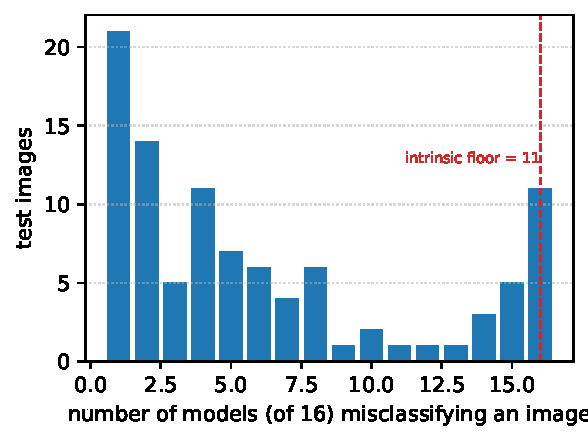
\includegraphics[width=\linewidth]{figures/error_floor.pdf}
    \caption{Images missed by exactly $k$ of the 16 models.
      Eleven are missed by all 16 simultaneously---an irreducible floor.}
    \label{fig:floor}
  \end{subfigure}\hfill
  \begin{subfigure}[t]{0.48\linewidth}
    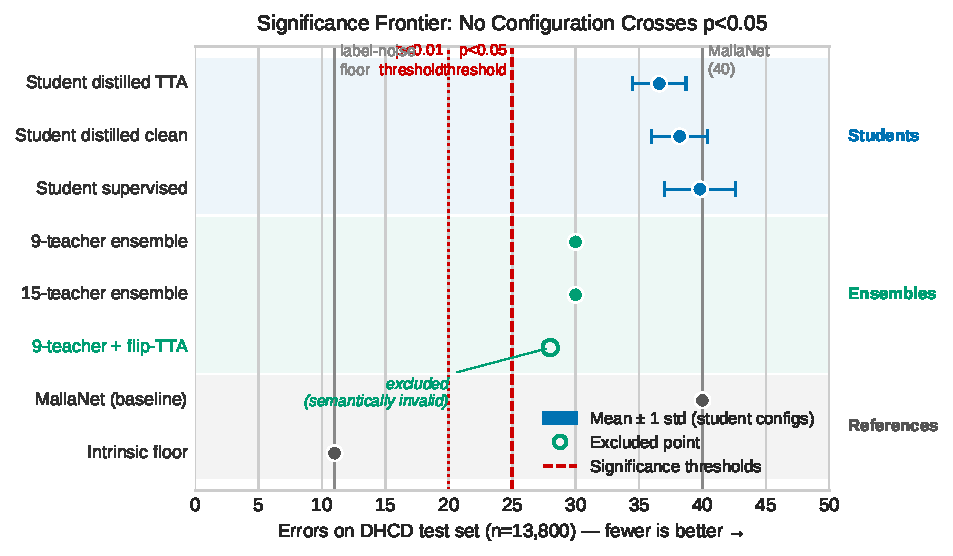
\includegraphics[width=\linewidth]{figures/significance_frontier.pdf}
    \caption{Every configuration sits above the $p{<}0.05$ threshold
      (25 errors). The 11-error floor marks the hard lower bound.}
    \label{fig:sig-frontier}
  \end{subfigure}
  \caption{Left: shared error floor across all 16 models.
    Right: significance frontier---30-error clean ensemble and 36.6-error
    student mean both lie in the statistical parity region.}
\end{figure}

When the same 11-image floor catches both a 1.11\,M-parameter compact
student and a baseline fifteen times its size, the problem is in the data.
Outside this floor, errors are model-specific (mean pairwise Jaccard
similarity $\mathbf{0.48}$): seeds shuffle which images fail, but
ensembling or adding seeds reduces \emph{variance}, not the \emph{bias} the
floor imposes.

\subsection{Confusable Character Pairs}

Script-level collisions dominate remaining mistakes.  Table~\ref{tab:confusions} lists
the top distilled-student confusion pairs aggregated across the 10
distilled seeds.  \textbf{ba / waw} leads with 17 cross-confusions, followed by
\textbf{waw / tabala} (16) and \textbf{tra / ba} (15); \textbf{dha / gha}
(13 instances) and \textbf{da / dhaa} (9 instances) round out the top five.

\begin{table}[t]\centering
\caption{Top confusion pairs in the distilled student pool (aggregate
  across 10 distilled seeds on the DHCD test set).}
\label{tab:confusions}
\begin{tabular}{lcc}\toprule
Pair & Cross-confusions & Script note \\\midrule
ba $\leftrightarrow$ waw    & 17 & Near-identical body, open vs.\ closed loop \\
waw $\leftrightarrow$ tabala & 16 & Shared curved baseline \\
tra $\leftrightarrow$ ba    & 15 & Conjunct ligature vs.\ simple consonant \\
dha $\leftrightarrow$ gha   & 13 & Looped ascender, subtle body curvature \\
da $\leftrightarrow$ dhaa   & 9  & Single hairline distinguishes the pair \\\bottomrule
\end{tabular}
\end{table}

These pairs expose a resolution limit: the confusable glyphs differ by
strokes finer than a few pixels at $32{\times}32$ resolution, and DHCD
provides neither higher-resolution inputs nor stroke-level annotation.

\subsection{Significance Frontier}
\label{sec:sig-frontier}

Under the exact two-sided McNemar test~\cite{mcnemar1947} at $\alpha = 0.05$,
crossing from statistical parity to a demonstrable improvement over the
reproduced baseline (40 errors) requires at most \textbf{25 errors}
($\geq$99.82\% accuracy) --- fewer than 15 additional correct classifications
separating inconclusive from significant.  A comfortable margin would require
$\leq$\textbf{20 errors} ($\geq$99.855\%), a target that demands
near-perfect resolution of the ambiguous-glyph pairs in
Table~\ref{tab:confusions}.

Every configuration tested stops just short of this frontier.  The best
single result is \textbf{28 errors}: the 9-teacher ensemble with
(semantically invalid) flip-TTA applied at test time, a result excluded
on methodological grounds (Section~\ref{sec:flip-tta}).  The best
defensible single seed reaches \textbf{34 errors}; the best ensemble
without flip-TTA reaches \textbf{30 errors}.  Both sit within the parity
region, separated from significance by the 11-image irreducible floor itself.

\textbf{No lever tested in this study achieved a statistically
significant improvement over the baseline.}  Scaling the teacher pool from 9
to 15, applying TTA-softened distillation targets, and running five
independent seeds all leave configurations outside the significance
frontier.  This is not a failure of experimental design---it defines a
saturated benchmark.  The significance frontier is not a line researchers
are approaching asymptotically, but a wall built from mislabelled images
and inherently ambiguous glyphs.


\subsection{Calibration}

Expected Calibration Error (ECE)~\cite{guo2017calibration} falls in the
range \textbf{0.13--0.16} across all \modelname{} configurations ---
unremarkable values for softmax classifiers without post-hoc temperature
scaling.  ECE does not co-vary with accuracy across seeds: better seeds are
not better calibrated.  Critically, the 11 floor images are confidently
wrong, not uncertain: models assign high probability to an incorrect class
on every seed, confirming the error floor is a data-level property that
architectural or training choices cannot correct.

\section{Discussion}
\label{sec:discussion}

\paragraph{Scope of transfer results.}
The transfer experiment (Section~\ref{sec:transfer}) covers only the
\textbf{digit subset} (10 of 46 DHCD classes).  Extending transfer to the
full 36-consonant inventory is not currently possible: the only publicly
available Devanagari handwriting collections that share DHCD's consonant
label taxonomy — principally the Acharya~\cite{acharya2015dhcd} and
Pant datasets — are same-provenance splits of DHCD itself, and using them
as held-out targets would reintroduce contamination between training and
evaluation.  Public literature does not yet provide genuinely independent
consonant-level benchmarks, so transferability claims are limited to
digits.  This constraint itself underscores a broader infrastructure gap:
the Devanagari recognition community currently lacks the diversity of
held-out corpora that would allow systematic transfer studies, and the
digit result — where the compact model outperforms a supervised baseline
by \textbf{+14\,pp} under domain shift — suggests such benchmarks would
be worth building.

\paragraph{Single-benchmark evaluation.}
All consonant-level accuracy results in this paper are reported on a
single held-out split of DHCD.  The McNemar test controls for
within-split variability via paired comparison, but without a second,
independent consonant benchmark the findings may not generalise beyond
this split.  The saturation conclusion depends on properties specific to
DHCD — its $32{\times}32$ resolution, its concentrated label noise, and
its writer pool — that another dataset might not share.  This is not a
weakness peculiar to this study; it reflects the current state of public
Devanagari corpora.  Readers should interpret the saturation claim as a
property of DHCD at this resolution and provenance, not necessarily of
Devanagari recognition as a problem class.

\paragraph{Efficiency versus accuracy.}
The \textbf{15.6$\times$} parameter reduction and \textbf{9.5$\times$}
latency improvement come at no measurable accuracy cost on DHCD at its
current saturation point.  This finding supports a general principle: on
saturated benchmarks, compactness is not a compromise but a rational
choice, since the errors that remain are inaccessible to any model
regardless of capacity.  Whether this efficiency advantage persists under
a more discriminative benchmark — one where larger models could exploit
additional capacity to push below the 11-error floor — is an open
question this work cannot answer.  These results therefore support
deployment on DHCD more directly than they support a general claim about
efficiency under harder conditions, and they motivate the construction of
such harder benchmarks as the most productive next step for the field.

\section{Conclusion}
\label{sec:conclusion}

The conclusion of saturation is unpleasant, but difficult to avoid. At the current resolution, the remaining errors in DHCD are driven more by label noise and handwriting ambiguities than by the model's ability. In other words, throwing a bigger recognizer at the problem does not buy a better recognizer. At that point, compactness is no longer a compromise. That will be the correct operating point.

\modelname{} reaches the accuracy of \textbf{99.73\,\%} with just the \textbf{1.11\,M} parameter and achieves statistical equivalence with the leading large-scale model baselines (McNemar $p = 0.345$) even before the advent of knowledge distillation. This means a parameter reduction of 15.6$\times$ and a CPU latency reduction of 9.5$\times$ without sacrificing accuracy. Why can't we move forward? The same \textbf{11-error} intrinsic floor breaks all tested configurations (including large-scale teacher ensembles), and ablation closes off the obvious escape route. Distillation target cleanliness, ensemble size, and test-time augmentation all have no statistically significant benefit. The floor is the ceiling.

The boundaries between the two must be clearly marked. The saturation claim is tied to certain conditions of DHCD, namely $32{\times}32$ resolution, concentrated label noise, and its particular pool of writers. Cleaner or higher resolution benchmarks may reveal capacity differences that DHCD may not reveal. The transfer results only cover \textbf{digit subset} (10 out of 46 classes). Consonant-level transferability is out of scope here, as there are no independent consonant target sets that share the label taxonomy of DHCD.

The practical implication for Devanagari recognition is to measure progress more honestly before claiming it. Without \emph{paired evaluation} -- McNemar or equivalent -- for a particular test case where the compared models also fail, a gain of a few hundredths of a percent is meaningless. The benchmark problem is even more difficult. DHCD served as a discriminator. The next necessary step is high-resolution scanning or a completely independent pool of writers.

\bibliographystyle{splncs04}
\bibliography{refs}
\end{document}
